\documentclass{article}
\usepackage{graphicx} % Required for inserting images
\usepackage[a4paper, total={6.5in, 9.5in}]{geometry}
\usepackage{amsmath}

\title{CTA200 Assignment 3}
\author{Ethan Kwan}
\date{May 8 2026}

\begin{document}

\maketitle

\section{The Mandelbrot Set}
\subsection{diverge\_when(c, z0=0, max\_iter=30)}
Finds whether a given point c on the complex plane converges or diverges after iterating through the sequence $z_{i+1} = z_{i}^2 + c$.

Parameters:
\begin{itemize}
    \item c: \textit{complex} \\
    The point on the complex plane.
    \item z0: \textit{float, optional} \\
    The first term of the sequence.
    \item max\_iter: \textit{int, optional} \\
    The maximum number of terms to calculate before a verdict is reached.
\end{itemize}

Returns:
\begin{itemize}
    \item n: \textit{int} \\
    The number of iterations it took for the sequence to diverge. Divergence defined as $||z_i|| > 100$. If the point does not diverge, then returns None.
\end{itemize}
\subsection{combine(real, imag)}
Takes the real part and the imaginary part of a complex number and combines them into the whole complex number.

Parameters:
\begin{itemize}
    \item real: \textit{array-like} \\
    The real part of the complex number.
    \item imag: \textit{array-like} \\
    The imaginary part of the complex number.
\end{itemize}

Returns:
\begin{itemize}
    \item c\_num: \textit{array-like} \\
    The whole complex number.
\end{itemize}
\subsection{Plots and result}
\begin{figure}[h]
    \centering
    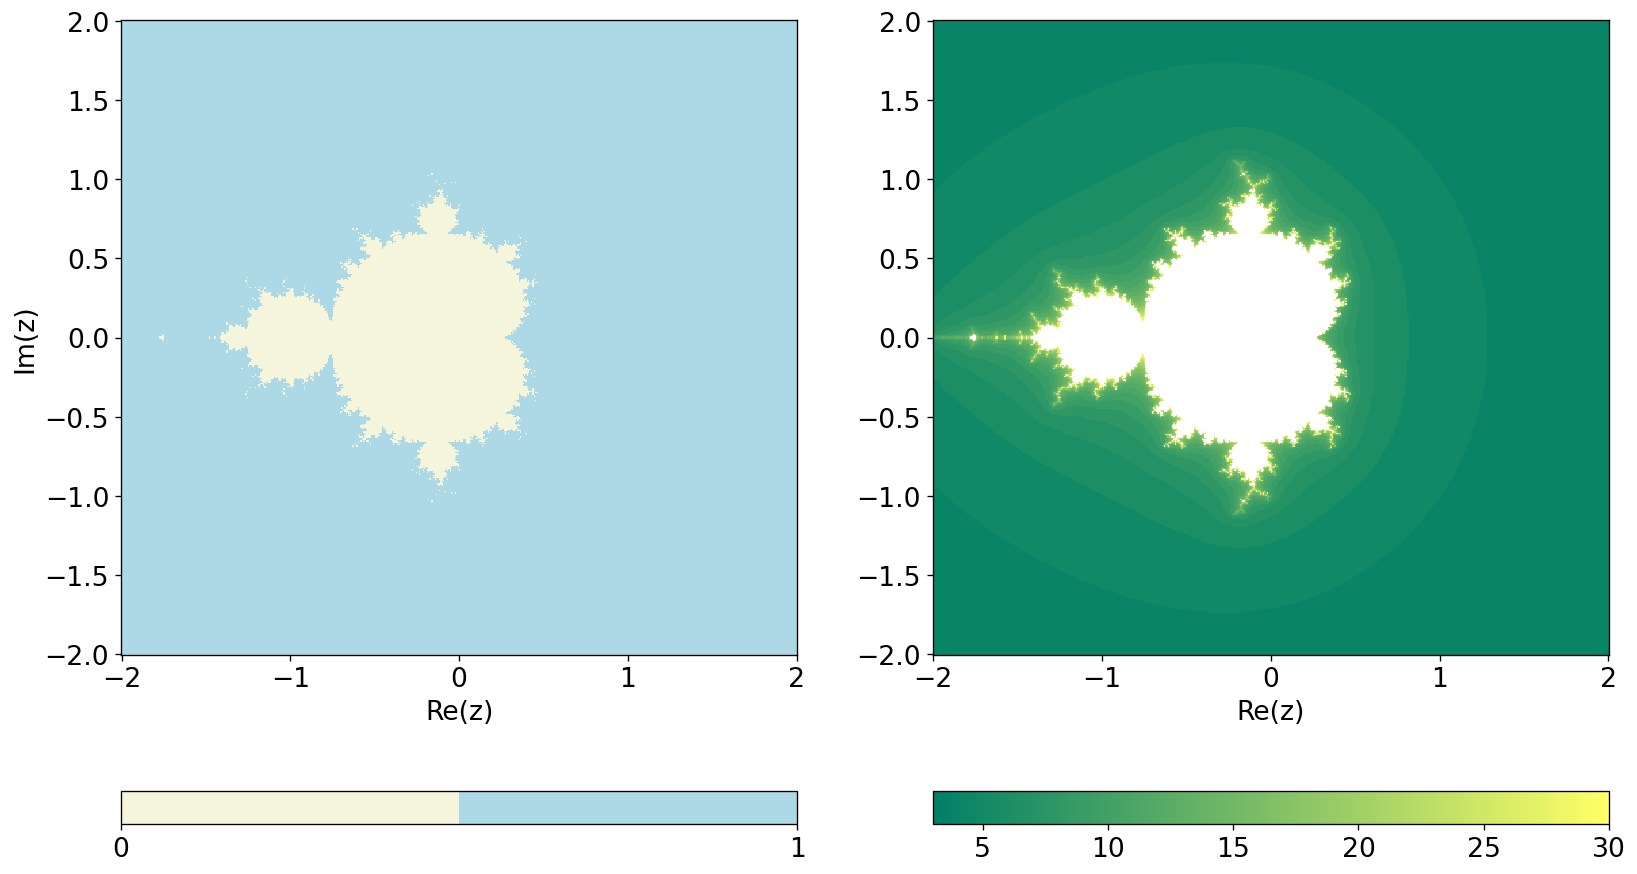
\includegraphics[width=1\linewidth]{mandelbrot.png}
    \caption{The Mandelbrot set, coloured two different ways. Left: coloured according to whether each point diverges or is bounded. On the colourbar, 0 corresponds to bounded and 1 corresponds to diverging. Right: coloured according to how fast each point diverges. White corresponds to no divergence, and the colourbar denotes how many terms of the sequence it took to diverge.}
    \label{fig:mandelbrot}
\end{figure}
This is the well-known Mandelbrot set. Figure \ref{fig:mandelbrot} displays the set coloured two different ways, one for whether each point diverges and the other for how fast each point diverges.
\section{Lorenz Systems}
\subsection{lorenz(t, v, sigma, r, b)}
Vectorized system of Lorenz equations used for the right-hand side of solve\_ivp. Uses the following three first-order differential equations:
\begin{align}
    \dot X&=-\sigma(X-Y)\\
    \dot Y&=rX-Y-XZ\\
    \dot Z&=-bZ+XY
\end{align}

Parameters:
\begin{itemize}
    \item t: \textit{array-like} \\
    Time.
    \item v: \textit{array-like} \\
    The vectorized coordinates [X, Y, Z].
    \item sigma: \textit{float} \\
    The Prandtl number, defined as the ratio of the kinematic viscosity to the thermal diffusivity.
    \item r: \textit{float} \\
    The Rayleigh number.
    \item b: \textit{float} \\
    The length scale.
\end{itemize}

Returns:
\begin{itemize}
    \item vdot: \textit{array-like} \\
    The vectorized time derivatives $[\dot X, \dot Y, \dot Z]$.
\end{itemize}
\subsection{distance(r, r\_p)}
Find the distance between two points r and r\_p.

Parameters:
\begin{itemize}
    \item r: \textit{array-like} \\
    The first coordinate point.
    \item r\_p: \textit{array-like} \\
    The second coordinate point.
\end{itemize}

Returns:
\begin{itemize}
    \item d: \textit{float} \\
    The distance between the two points.
\end{itemize}
\subsection{Plots and result}
Figures \ref{fig:lorenz 1} and \ref{fig:lorenz 2} are reproductions from Lorenz' paper. I hypothesize that their slight incongruence to Lorenz' figures are likely due to a difference in numerical solver. Lorenz' plotted solution to the convection equations seems to evolve for longer than ours, which may mean that his timestep was greater.

Figure \ref{fig:lorenz dev} displays the distance between two solutions with only slightly differing initial conditions. We see on the semilog plot that a difference of 1e-8 in only one coordinate causes the distance between solutions to grow exponentially, leaving the end states of each solution very far apart in phase space.
\begin{figure}[h]
    \centering
    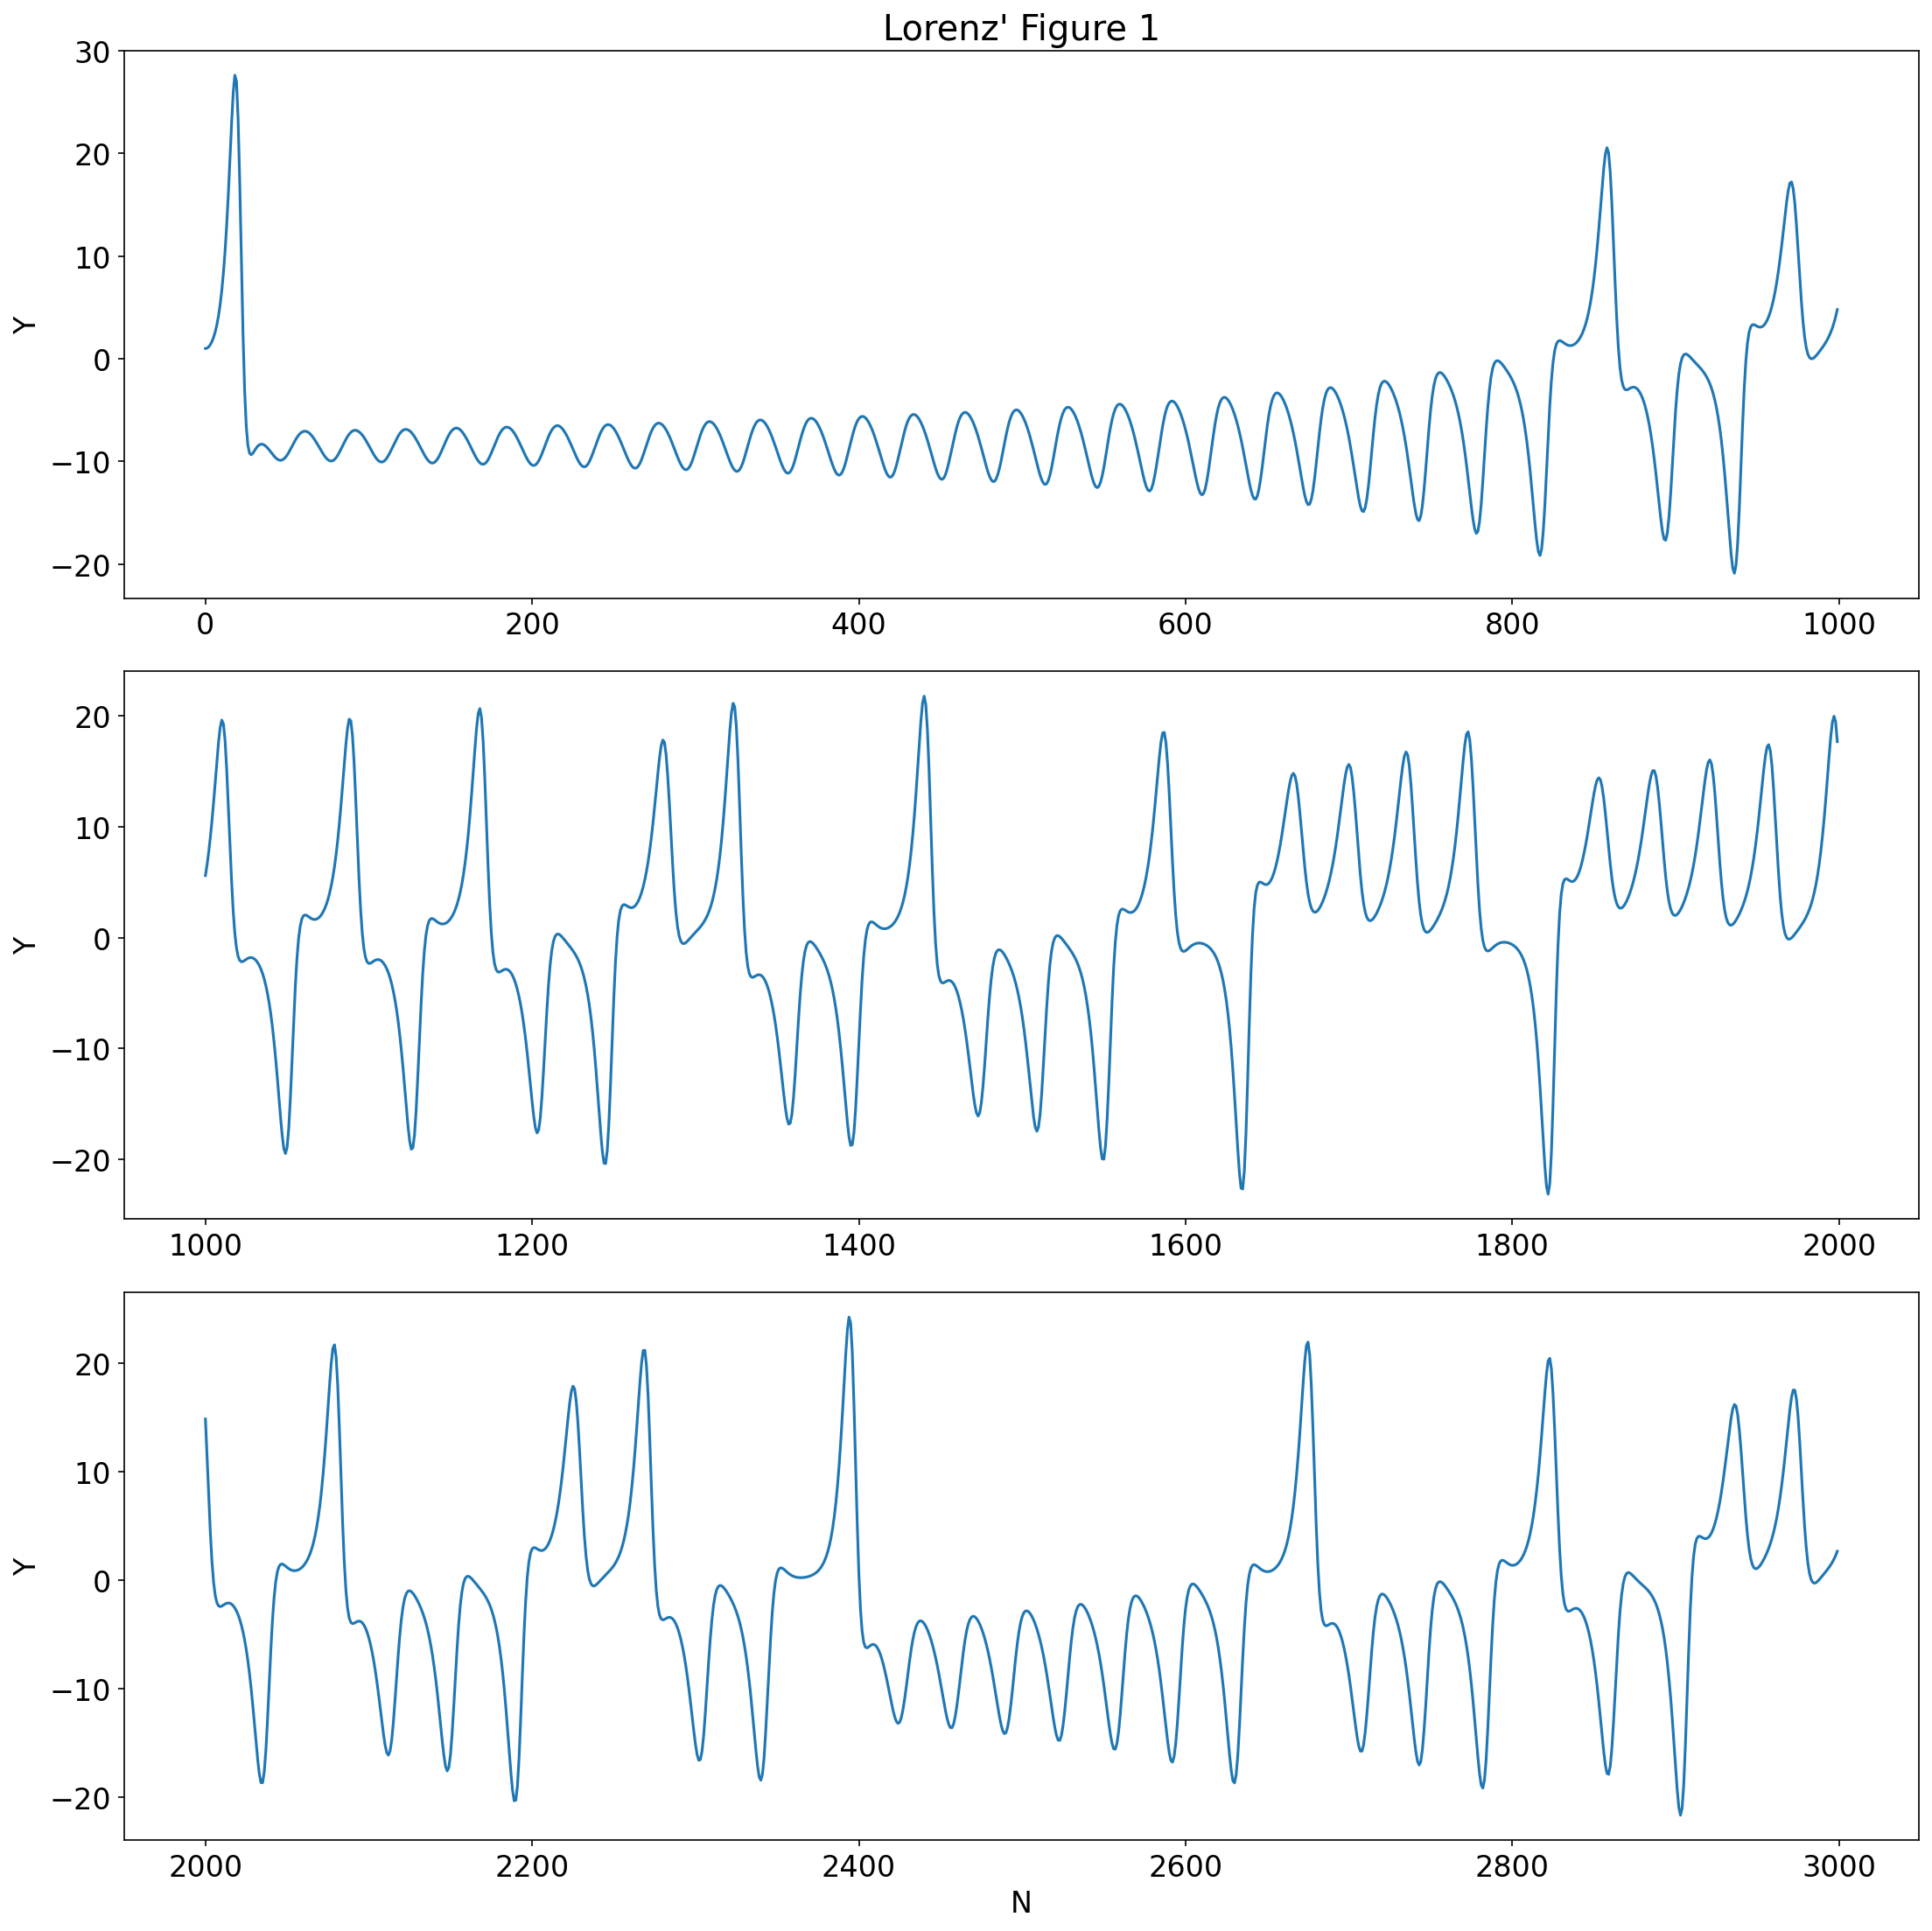
\includegraphics[width=0.75\linewidth]{lorenz 1.png}
    \caption{Reproduced Figure 1 from Lorenz' paper. Numerical solution of the convection equations. First 60 units of time are shown.}
    \label{fig:lorenz 1}
\end{figure}
\begin{figure}[h]
    \centering
    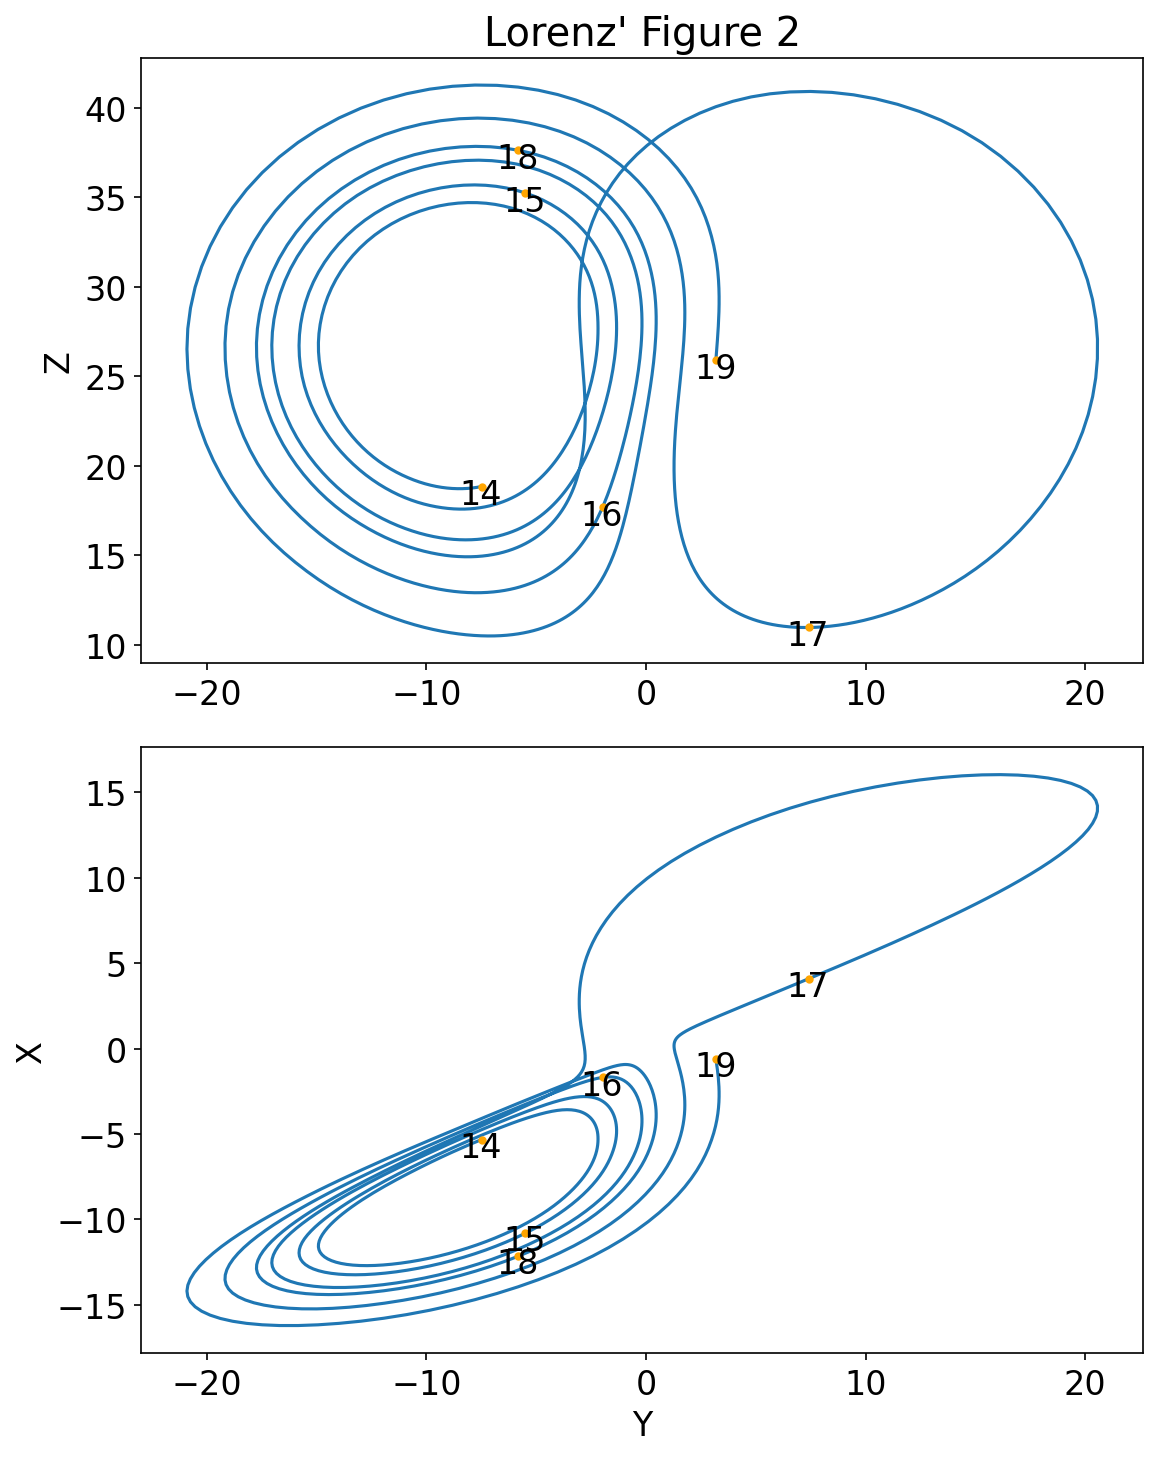
\includegraphics[width=0.75\linewidth]{lorenz 2.png}
    \caption{Reproduced Figure 2 from Lorenz' paper. Numerical solution of the convection equations. Projections on the Y-Z and X-Y planes of phase space are shown for the time interval 14-19.}
    \label{fig:lorenz 2}
\end{figure}
\begin{figure}[h]
    \centering
    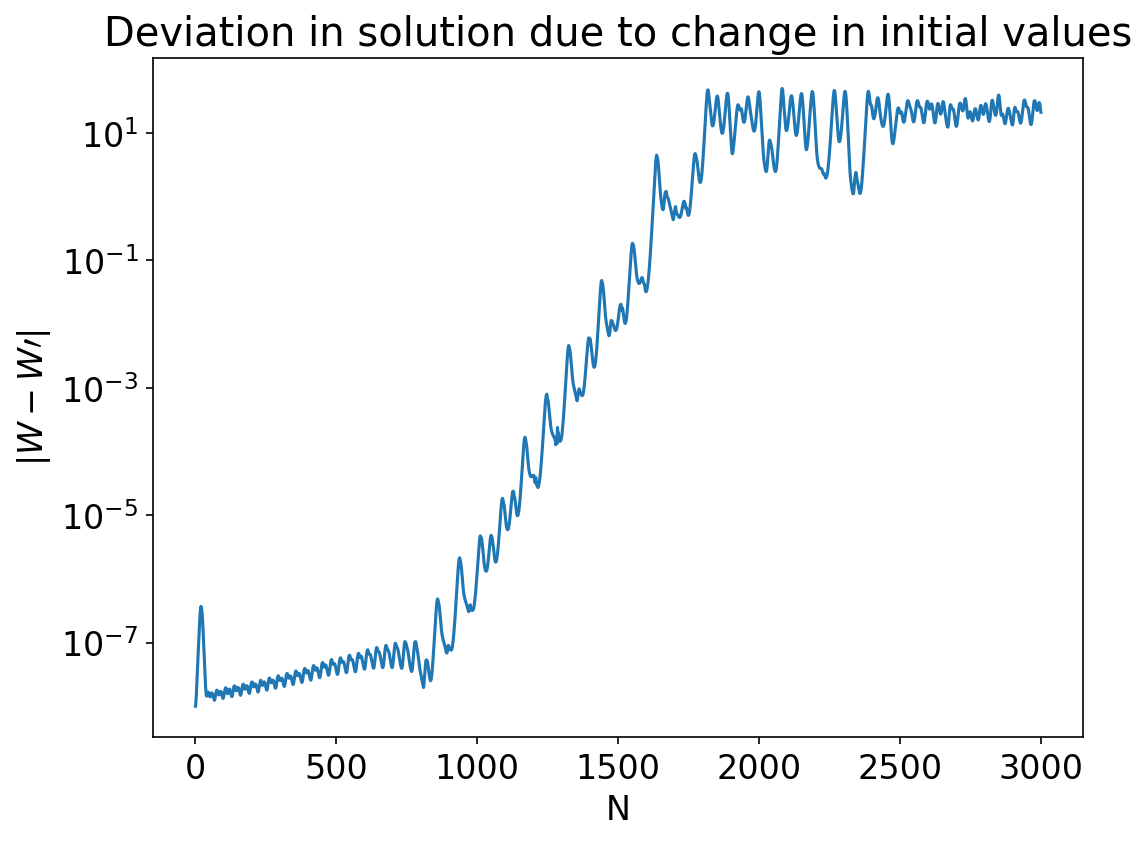
\includegraphics[width=1\linewidth]{lorenz dev.png}
    \caption{Distance between two solutions two the convection equations with slightly different initial conditions. Fiducial solution has initial conditions [X, Y, Z] = [0, 1, 0] and primed solution has initial conditions [X, Y, Z] = [0, 1 + 1e-8, 0]. Plotted on semilog axes (linear x-axis, log y-axis) such that the exponential growth in distance is observable.}
    \label{fig:lorenz dev}
\end{figure}
\end{document}
